\chapter{Il problema dei due corpi}
\label{chap:due-corpi}

In questo capitolo affronteremo il \emph{problema dei due corpi}, cioè lo studio
del moto di due corpi, supposti puntiformi, soggetti solamente alla mutua
interazione dovuta a forze che soddisfano il principio di azione e reazione. In
particolare ci occuperemo del \emph{problema di Keplero}, ovvero del caso in cui
la forza fra i due corpi è quella gravitazionale, o più in generale dipendente
dall'inverso del quadrato della distanza fra i due corpi, che è di tipo
centrale. Il problema sarà risolto usando il formalismo newtoniano (si vedano
\textcites{bradt:processes}{fabrizio:meccanica}{smart:textbook}) e quelli
lagrangiano e hamiltoniano (si vedano
\textcites{goldstein:meccanica}{landau:meccanica}), di questi ultimi daremo una
breve presentazione. Riusciremo a determinare analiticamente le equazioni delle
orbite dei due corpi e a dedurre alcune proprietà del sistema. La risoluzione
del problema di Keplero permette di descrivere, fra le altre cose, il moto di
due corpi celesti, per esempio un pianeta e la sua stella, che sono soggetti
solo alla mutua interazione gravitazionale.

\section{Formalismo newtoniano}
\label{sec:formalismo-newton}

\begin{figure}
  \centering
  \begin{tikzpicture}[font=\footnotesize,scale=3]
    % m1=1: y=0.8,  z=0.2,  x=0.2
    % m2=3: y=0.6,  z=0.8,  x=0.4
    % cm:   y=0.65, z=0.65, x=0.35
    \node [inner sep=0](O) at (0,0,0) [label=left:$O$] {};
    \draw [->] (O) -- (1,0,0) node[right] {$y$}; % asse y
    \draw [->] (O) -- (0,1,0) node[above] {$z$}; % asse z
    \draw [->] (O) -- (0,0,1) node[below left] {$x$}; % asse x
    \filldraw [gray] (0.8,0.2,0.2) circle (0.01); % corpo di massa m_2
    \draw [->] (0,0,0) -- node[below right,fill=white] {$\bm{r}_2$}
               (0.8,0.2,0.2) node[right] {$m_2$}; % vettore r_2
    \filldraw [gray] (0.6,0.8,0.4) circle (0.02); % corpo di massa m_1
    \draw [->] (0,0,0) -- node[above left] {$\bm{r}_1$} (0.6,0.8,0.4)
               node[above] {$m_1$}; % vettore r_1
    % vettore posizione relativa
    \draw [<-] (0.8,0.2,0.2) -- node[right] {$\bm{r}$} (0.6,0.8,0.4);
    % vettore posizione del centro di massa
    \draw [->] (0,0,0) -- node[right] {$\bm{r}_\textup{CM}$} (0.65,0.65,0.35);
  \end{tikzpicture}
  \caption{Due corpi in un sistema di riferimento inerziale}
  \label{fig:due-corpi}
\end{figure}
Consideriamo un sistema costituito da due corpi puntiformi, di masse $m_1$ e
$m_2$ e in un fissato sistema di riferimento inerziale indichiamo con $\bm{r}_1$
e $\bm{r}_2$ i rispettivi vettori posizione, come nella
Figura~\ref{fig:due-corpi}. Per la seconda legge di Newton, la forza
$\bm{F}_{21}$ che il corpo di massa $m_1$ esercita sul corpo di massa $m_2$ è
data da
\begin{equation}
  \label{eq:f21}
  \bm{F}_{21} = m_2\toder[2]{\bm{r}_2}{t}
\end{equation}
e la forza $\bm{F}_{12}$ che il corpo di massa $m_2$ esercita sull'altro è
\begin{equation}
  \label{eq:f12}
  \bm{F}_{12} = m_1\toder[2]{\bm{r}_1}{t}.
\end{equation}
Assumiamo per ipotesi che queste due forze soddisfino il principio di azione e
reazione nella forma forte:
\begin{equation}
  \label{eq:azione-reazione}
  \bm{F}_{12} = -\bm{F}_{21}.
\end{equation}
Definiamo il vettore \emph{posizione relativa}
\begin{equation}
  \label{eq:posizione-relativa}
  \bm{r}=\bm{r}_2-\bm{r}_1
\end{equation}
e il vettore posizione del \emph{centro di massa}
\begin{equation}
  \label{eq:centro-di-massa}
  \bm{r}_\textup{CM} = \frac{m_1\bm{r}_1+m_2\bm{r}_2}{m_1+m_2}.
\end{equation}
Dalle equazioni~\eqref{eq:posizione-relativa} e~\eqref{eq:centro-di-massa}
possiamo ricavare $\bm{r}_1$ e $\bm{r}_2$ in funzione di $\bm{r}$ e
$\bm{r}_\textup{CM}$:
\begin{subequations}
  \label{eq:r1-r2-posizione-relativa-cdm}
  \begin{align}
    \bm{r}_1 &= \bm{r}_\textup{CM} - \frac{m_2}{m_1+m_2}\bm{r} =
    \bm{r}_\textup{CM} - \frac{\mu}{m_1}\bm{r},\\
    \bm{r}_2 &= \bm{r}_\textup{CM} + \frac{m_1}{m_1+m_2}\bm{r} =
    \bm{r}_\textup{CM} + \frac{\mu}{m_2}\bm{r},
  \end{align}
\end{subequations}
in cui abbiamo introdotto la \emph{massa ridotta} $\mu$ definita dalla metà
della media armonica fra $m_1$ e $m_2$
\begin{equation}
  \frac{1}{\mu} = \frac{1}{m_1} + \frac{1}{m_2} \iff \mu=\frac{m_1m_2}{m_1+m_2}.
\end{equation}
Osserviamo che la massa ridotta è sempre minore delle due masse, infatti
\begin{equation}
  \mu =\frac{m_1}{m_1/m_2+1} = \frac{m_2}{1+m_2/m_1},
\end{equation}
quindi $\mu < m_1,m_2$ per qualsiasi valore positivo delle due masse. Definiamo
inoltre la \emph{massa totale} $M_\textup{T}$ del sistema
\begin{equation}
  M_\textup{T}=m_1+m_2.
\end{equation}
Dalle definizioni di massa ridotta e totale deriva che
$M_\textup{T}\mu=m_1m_2$. Se, per esempio, $m_1\gg m_2$, allora $\mu\simeq m_2$ e
$M_\textup{T}\simeq m_1$. L'equazione del moto del centro di massa può essere
trovata semplicemente calcolando l'accelerazione di $\bm{r}_\textup{CM}$:
\begin{equation}
  \toder[2]{\bm{r}_\textup{CM}}{t} = \frac{1}{M_\textup{T}}
  \left(
    m_1\toder[2]{\bm{r}_1}{t} + m_2\toder[2]{\bm{r}_2}{t}
  \right) = \frac{\bm{F}_{12}+\bm{F}_{21}}{M_\textup{T}} = \bm{0},
\end{equation}
cioè il centro di massa è in quiete o si muove di moto rettilineo
uniforme. Poiché il sistema in cui il centro di massa è a riposo è un sistema
inerziale, questo può essere scelto come nostro nuovo sistema di riferimento.
In particolare, fissiamo come origine del sistema il centro di massa. In questo
nuovo sistema le posizioni delle due masse saranno dunque descritte dai vettori
\begin{subequations}
  \label{eq:r1-r2-nel-cdm}
  \begin{align}
    \bm{r}_1 &= -\frac{\mu}{m_1}\bm{r}, \label{eq:r1-nel-cdm}\\
    \bm{r}_2 &= \frac{\mu}{m_2}\bm{r}.
  \end{align}
\end{subequations}
Osserviamo che se, per esempio, $m_1\gg m_2$, allora $\bm{r}_1\simeq\bm{0}$,
cioè il corpo più massivo si trova praticamente nel centro di massa, come è
logico aspettarsi dalla definizione di centro di massa.

Dividendo ambo i membri della~\eqref{eq:f21} per $m_2$, ambo i membri
della~\eqref{eq:f12} per $m_1$ e sottraendo membro a membro le equazioni così
ottenute ricaviamo
\begin{equation}
  \frac{\bm{F}_{21}}{m_2}-\frac{\bm{F}_{12}}{m_1} = \bm{F}_{21}
  \left(
    \frac{1}{m_2}+\frac{1}{m_1}
  \right) = \frac{\bm{F}_{21}}{\mu} = \toder[2]{(\bm{r}_2-\bm{r}_1)}{t} =
  \toder[2]{\bm{r}}{t}
\end{equation}
in cui abbiamo ricordato che vale il principio di azione e reazione espresso
dalla~\eqref{eq:azione-reazione}. L'equazione precedente può essere riscritta
nella forma
\begin{equation}
  \label{eq:f21-mu}
  \bm{F}_{21}=\mu\toder[2]{\bm{r}}{t}
\end{equation}
da cui possiamo dedurre che il problema del moto relativo dei due corpi si è
ridotto allo studio del moto di un solo corpo fittizio, che chiameremo
\emph{particella relativa}, di massa $\mu$ all'interno del campo generato da un
altro corpo fittizio puntiforme di massa $M_\textup{T}$ e fisso, istante per
istante, nella posizione di uno dei due corpi. Poiché nel nostro caso abbiamo
definito la posizione relativa come $\bm{r}=\bm{r}_2 - \bm{r}_1$, abbiamo che il
corpo fittizio di massa pari alla massa totale occupa la posizione del corpo
reale di massa $m_1$. Istante per istante il vettore $\bm{r}$ indica la
posizione della particella fittizia $\mu$ nel sistema di riferimento di
$M_\textup{T}$.

\subsection{Problema di Keplero}
\label{sec:problema-keplero}

Consideriamo il caso dell'interazione gravitazionale. Se indichiamo con $M$ la
massa del corpo che genera il campo a cui è soggetto un corpo di massa $m$ e con
$\bm{r}$ il vettore diretto dal corpo di massa $M$ verso il corpo di massa $m$,
allora la forza $\bm{F}_\textup{G}$ agente su $m$ è data da
\begin{equation}
  \label{eq:legge-attrazione}
  \bm{F}_\textup{G} = -\frac{GMm}{r^2}\versor{r},
\end{equation}
in cui $G=\SI{6.673 84(80)e-11}{\cubic\metre\per\kilogram\per\second\squared}$ è
la costante di gravitazione universale (il valore della costante è preso da
\textcite{codata:costanti}). Si tratta di una forza centrale, cioè puramente
radiale, e il segno meno indica che è sempre attrattiva verso il centro del
campo. Sostituendo la~\eqref{eq:legge-attrazione} nella~\eqref{eq:f21-mu}
abbiamo
\begin{equation}
  \label{eq:forza-mu}
  \bm{F}_{21} = -\frac{GM_\textup{T}\mu}{r^2}\versor{r} =
  -\frac{Gm_1m_2}{r^2}\versor{r} = \mu\toder[2]{\bm{r}}{t}.
\end{equation}

Per una qualsiasi forza di tipo centrale il momento angolare $\bm{l} = \bm{r}
\times \bm{p}$ rispetto al centro della forza è una costante del moto. Infatti
il momento torcente $\bm{\tau}$ di una forza $\bm{F}$ rispetto a un polo $O$ è
definito da
\begin{equation}
  \bm{\tau}= \toder{\bm{l}}{t} = \bm{r}\times\bm{F}.
\end{equation}
Qui con $\bm{r}$ indichiamo il vettore congiungente il polo con il punto di
applicazione della forza. Poiché la forza $\bm{F}$ è radiale, il momento
torcente associato è nullo, implicando quindi la costanza nel tempo del momento
angolare $\bm{l}$ calcolato rispetto allo stesso polo.

Ritornando al problema di Keplero, abbiamo appena visto che il momento angolare
della particella di massa ridotta rispetto alla posizione di $M_\textup{T}$ è un
integrale primo del moto. Notiamo ora che, per definizione di momento angolare,
i vettori $\bm{r}$ e $\bm{l}\equiv\bm{l}_0$ sono fra loro perpendicolari. Allora
la costanza del vettore $\bm{l}_0$, e in particolare della sua direzione,
implica che, nel caso $\bm{l}_0\neq\bm{0}$, il vettore $\bm{r}$, giace sempre
sullo stesso piano perpendicolare a $\bm{l}_0$. Se invece risulta
$\bm{l}_0=\bm{0}$, $\bm{r}$ è parallelo alla quantità di moto $\bm{p}$ e il moto
è unidimensionale. Da qui in seguito supporremo che il momento angolare
$\bm{l}_0$ della particella relativa sia non nullo.

Dal momento che il moto della particella di massa ridotta si svolge in un piano,
possiamo utilizzare le coordinate polari $r,\theta$ per rappresentare la
posizione del corpo nel sistema di riferimento di $M_\textup{T}$. Dalla
meccanica si ricava che per un moto piano la velocità $\dot{\bm{r}}$ e
l'accelerazione $\ddot{\bm{r}}$ del vettore posizione $\bm{r}=r\versor{r}$ sono
date da
\begin{subequations}
  \begin{align}
    \dot{\bm{r}}  &= \dot{r}\versor{r} +
    r\dot{\theta}\versor{\theta}, \label{eq:velocita-polare}\\
    \ddot{\bm{r}} &= (\ddot{r}-r\dot{\theta}^2)\versor{r} + (r\ddot{\theta} +
    2\dot{r}\dot{\theta}) \versor{\theta}.
  \end{align}
\end{subequations}
Usando le coordinate polari, l'equazione vettoriale~\eqref{eq:forza-mu} può
essere riscritta come due equazioni scalari:
\begin{subequations}
  \begin{gather}
    -\frac{GM_\textup{T}\mu}{r^2} = \mu(\ddot{r} - r\dot{\theta}^2) \iff
    -\frac{GM_\textup{T}}{r^2}=\ddot{r}-r\dot{\theta}^2,
    \label{eq:forza-mu-radiale}\\
    0 = \mu(r\ddot{\theta} +
    2\dot{r}\dot{\theta}). \label{eq:forza-mu-azimutale}
  \end{gather}
\end{subequations}
Dalla~\eqref{eq:forza-mu-azimutale} si trova nuovamente la costanza del modulo
$l_0 = \norm{\bm{l}_0} = \mu r^2\dot{\theta}$ del momento angolare. Infatti
\begin{equation}
  0 = r\mu(r\ddot{\theta} + 2\dot{r}\dot{\theta}) = \toder{\mu
    r^2\dot{\theta}}{t} = \toder{l_0}{t}.
\end{equation}

\begin{figure}
  \centering
  \begin{tikzpicture}[font=\footnotesize,scale=2]
    \draw[->] (0.6,1.2) .. controls (0.8,1.19) and (1.1,1.196) .. (1.299,0.75)
                        .. controls (1.5,0.3)  and (1.7,0.2)   .. (2.0,0.0)
                        .. controls (2.3,-0.2) and (2.4,-0.2)  .. (2.6,-0.3);
    \draw (0,0) node[left] {$O$};
    \draw[->] (0,0) -- node[below] {$r+\dd r$} (2,0);
    \draw[->] (0,0) -- node[above] {$r$} (1.299,0.75);
    \draw[dashed] (1.299,0) -- node[left] {$r\dd\theta$} (1.299,0.75);
    \draw[->] ($0.4*cos(30)*(1,0)+ 0.4*sin(30)*(0,1)$) to [out=-60,in=90]
              node[right] {$\dd\theta$} (0.4,0);
  \end{tikzpicture}
  \caption[Area spazzata nell'intervallo di tempo $\dd t$ dal vettore
  posizione]{Area spazzata nell'intervallo di tempo $\dd t$ dal vettore
    posizione di un corpo in moto lungo una traiettoria generica}
\label{fig:area-differenziale}
\end{figure}
L'area differenziale $\dd A$ spazzata dalla particella di massa ridotta che si
sposta di un angolo infinitesimo $\dd\theta$ è espressa da (si veda la
Figura~\ref{fig:area-differenziale})
\begin{equation}
  \dd A = \frac{r\cdot r\dd\theta}{2} = \frac{r^2\dd\theta}{2},
\end{equation}
quindi la velocità areolare $\ltoder{A}{t}$ è
\begin{equation}
  \label{eq:velocita-areolare}
  \toder{A}{t} = \frac{1}{2}r^2\dot{\theta} = \frac{1}{2}\frac{l_0}{\mu} =
  \text{costante}.
\end{equation}
Abbiamo così ottenuto la seconda legge di Keplero: \emph{il vettore posizione
  della particella rispetto al centro dell'orbita (o della forza) spazza aree
  uguali in intervalli di tempo uguali}. Osserviamo che per giungere a questo
risultato è stato sufficiente utilizzare la costanza del momento angolare che
deriva a sua volta dal carattere centrale della forza; pertanto questa legge
è valida per tutte le forze di questo tipo.

\subsection{Equazione dell'orbita}
\label{sec:equazione-dellorbita}

Nel problema di Keplero, vogliamo ora cercare un'espressione esplicita della
coordinata polare $r$ in funzione dell'altra coordinata $\theta$, che a sua
volta dipenderà dal tempo. Per fare ciò è conveniente effettuare la sostituzione
$u=1/r$. Calcolando le derivate temporali di $r$ otteniamo che
\begin{subequations}
  \begin{align}
    \dot{r} &= \toder{r}{t} = \toder{r}{\theta}\toder{\theta}{t} =
    \toder{(1/u)}{\theta}\dot{\theta} =
    -\frac{\dot{\theta}}{u^2}\toder{u}{\theta}
    = -\frac{l_0}{\mu}\toder{u}{\theta}, \label{eq:derivata1-r}\\
    \begin{split}
      \ddot{r} &= \toder[2]{r}{t} = \toder{}{\theta}
      \left( \toder{r}{t} \right)\toder{\theta}{t} = \toder{}{\theta}
      \left( -\frac{l_0}{\mu}\toder{u}{\theta} \right)\dot{\theta} =
      -\frac{l_0\dot{\theta}}{\mu}\toder[2]{u}{\theta} \\
      &= - \left( \frac{l_0}{\mu}
      \right)^2u^2\toder[2]{u}{\theta}. \label{eq:derivata2-r}
    \end{split}
  \end{align}
\end{subequations}
Sostituendo la~\eqref{eq:derivata2-r} nella~\eqref{eq:forza-mu-radiale} abbiamo
\begin{equation}
  -GM_\textup{T}u^2 = -
  \left(
    \frac{l_0}{\mu}
  \right)^2u^2\toder[2]{u}{\theta} - \frac{l_0^2u^3}{\mu^2}.
\end{equation}
Poiché $r$ rappresenta la distanza della particella di massa ridotta da
$M_\textup{T}$, essa assume valori finiti e il suo reciproco $u$ non è mai
nullo. Nell'equazione precedente possiamo quindi dividere ambo i membri per
$u^2$ ottenendo
\begin{equation}
  \toder[2]{u}{\theta} + u = \frac{GM_\textup{T}\mu^2}{l_0^2}.
\end{equation}
Questa è una equazione differenziale ordinaria lineare del secondo ordine a
coefficienti costanti, chiamata \emph{equazione di Binet}. Per semplificare i
calcoli poniamo
\begin{equation}
  \label{eq:reciproco-semilato}
  \frac{GM_\textup{T}\mu^2}{l_0^2} = \frac{1}{p},
\end{equation}
di modo che l'integrale generale dell'equazione di Binet diventa
\begin{equation}
  \label{eq:soluzione-binet}
  u(\theta) = c_0\cos\theta + c_1\sin\theta + \frac{1}{p},
\end{equation}
con $c_0$ e $c_1$ costanti di integrazione. Imponiamo le seguenti condizioni
iniziali
\begin{subequations}
  \label{eq:condizioni-binet}
  \begin{align}
    u(\theta_0) &= \frac{1+e}{p},\\
    \toder{u}{\theta}(\theta_0) &= 0,
  \end{align}
\end{subequations}
che significano richiedere che il punto $\theta = \theta_0$ sia stazionario per
la funzione $u(\theta)$ e che in questo punto la funzione $u$ assuma il valore
$(1+e)/p$. Vedremo più avanti il significato delle grandezze $e$ e
$p$. Osserviamo che queste condizioni equivalgono a richiedere
\begin{subequations}
  \begin{align}
    r(\theta_0) &= \frac{1}{u(\theta)} = \frac{p}{1+e}, \\
    \toder{r}{\theta}(\theta_0) &= \toder{(1/u)}{\theta}(\theta_0) =
    -\frac{1}{u^2(\theta_0)} \toder{u}{\theta}(\theta_0) = 0.
  \end{align}
\end{subequations}
Con le condizioni~\eqref{eq:condizioni-binet} le costanti di integrazione
valgono
\begin{subequations}
  \label{eq:costanti-binet}
  \begin{align}
    c_0 &= \frac{e}{p}\cos\theta_0, \\
    c_1 &= \frac{e}{p}\sin\theta_0,
  \end{align}
\end{subequations}
pertanto la soluzione dell'equazione di Binet~\eqref{eq:soluzione-binet} con le
condizioni~\eqref{eq:condizioni-binet} è
\begin{equation}
  \label{eq:soluzione2-binet}
  u(\theta) = \frac{1}{p}(1 + e\cos\theta\cos\theta_0 +
  e\sin\theta\sin\theta_0) =  \frac{1}{p}(1+e\cos(\theta-\theta_0)).
\end{equation}
Ricordando che $r(\theta)=1/u(\theta)$ giungiamo, infine, all'equazione polare
dell'orbita della particella relativa nel sistema di riferimento di
$M_\textup{T}$
\begin{equation}
  \label{eq:orbita}
  r(\theta) = \frac{p}{1+e\cos(\theta-\theta_0)}.
\end{equation}

\subsection{Classificazione geometrica delle orbite}
\label{sec:class-geom-orbite}

La~\eqref{eq:orbita} è l'equazione polare di una conica con centro nel fuoco o
uno dei fuochi nel caso dell'ellisse. La costante $e$ è chiamata
\emph{eccentricità} della conica, la costante $p$ invece è detta
\emph{semilato retto}. Entrambe possono assumere valori non negativi. La
quantità $\chi = \theta - \theta_0$ è chiamata \emph{anomalia vera} o
\emph{effettiva}. A seconda dei diversi valori dell'eccentricità le coniche
possono essere classificate nel seguente modo:
\begin{itemize}
\item $0\leq e<1$: \emph{ellisse}. Nel caso particolare $e=0$ si ha una
  \emph{circonferenza};
\item $e=1$: \emph{parabola};
\item $e>1$: \emph{iperbole}.
\end{itemize}
\begin{figure}
  \centering
  \begin{tikzpicture}[font=\scriptsize,scale=5]
    % a=1, e=0.8, b=a*sqrt(1-e^2)=0.6, c=a*e=0.8, p=a*(1-e^2)=0.36
    \draw[->] (-1.1,0) -- (1.1,0) node[right] {$x\equiv x'$}; %assi x e x'
    \draw[->] (0,-0.7) -- (0,0.7) node[above] {$y'$}; %asse y'
    \draw[->] (0.8,-0.7) -- (0.8,0.7) node[above] {$y$}; %asse y
    \draw (0,0) ellipse (1 and 0.6);
    \draw (0,0) node[below left] {$O'$};
    \draw (0.8,0) node[below left] {$O\equiv M_{\textup{T}}$};
    \draw[->] (0.9,0) to [out=90,in=-45] node[inner sep=0,fill=white,right=3]
              {$\theta - \theta_0$} ($(0.8,0) + cos(45)*(0.1,0) +
              sin(45)*(0,0.1)$);
    \draw[->] (0.8,0) -- node[above] {$r$} (0.962586,0.162586);
    \node [below] at ($(0,0)!.5!(-1,0)$) {$a$};
    \node [above] at ($(0,0)!.5!(0.8,0)$) {$c$};
    \node [left] at ($(0,0)!.5!(0,0.6)$) {$b$};
    \node [left] at ($(0.8,0)!.5!(0.8,0.36)$) {$p$};
    \node [below] at ($(0.8,0)!.5!(1,0)$) {$a-c$};
  \end{tikzpicture}
  \caption[Ellisse in coordinate polari]{Ellisse in coordinate polari. L'origine
    del sistema di riferimento $Oxy$ è la posizione di $M_\textup{T}$ e coincide
    con uno dei fuochi dell'ellisse, $a$ è il semiasse maggiore, $b$ è il
    semiasse minore, $p$ è il semilato retto, $c$ è l'eccentricità lineare. Il
    sistema di riferimento $O'x'y'$ ha origine nel centro dell'ellisse. Nel
    grafico abbiamo posto $a=1$ ed $e=0.8$}
  \label{fig:ellisse}
\end{figure}

Ricordiamo alcune proprietà geometriche delle coniche. Per l'ellisse (vedi la
Figura~\ref{fig:ellisse}) il semilato retto $p$ è dato da
\begin{equation}
  \label{eq:semilato-ellisse}
  p = a(1-e^2) = \frac{b^2}{a},
\end{equation}
dove $a$ è il \emph{semiasse maggiore} dell'ellisse e $b$ è il \emph{semiasse
  minore}. Dalla~\eqref{eq:semilato-ellisse} ricaviamo inoltre che
\begin{align}
  b &= a\sqrt{1-e^2}, \label{eq:semiasse-minore-ellisse}\\
  e &= \sqrt{1-\frac{b^2}{a^2}} =
  \sqrt{1-\frac{p}{a}}. \label{eq:eccentricita-ellisse}
\end{align}
L'\emph{eccentricità lineare} $c$ è la distanza fra il centro dell'ellisse e i
fuochi e risulta
\begin{equation}
  c=\sqrt{a^2-b^2} = ae.
\end{equation}
Il \emph{periapside} è il punto di un'ellisse più vicino a uno dei due fuochi,
l'\emph{apoapside} è il punto dell'ellisse più lontano dallo stesso
fuoco. Osservando la Figura~\ref{fig:ellisse} si riconosce che il periapside
rispetto al fuoco $M_\textup{T}$ è raggiunto in corrispondenza di
$\theta=\theta_0$, cioè quando l'anomalia vera $\chi$ è nulla, e la distanza del
periapside da $M_\textup{T}$ è $r_\textup{min} = r(\theta_0) = a(1-e) = a-c$;
l'apoapside è raggiunto per $\theta=\theta_0+\pi$, vale a dire quando l'anomalia
vera $\chi$ è uguale a $\pi$, e la distanza dell'apoapside dallo stesso fuoco è
$r_\textup{max} = r(\theta_0+\pi) = a(1+e)= a+c$. Si ottiene il caso particolare
della circonferenza ponendo nelle equazioni precedenti $e=0$, quindi $p=a=b$,
$c=e=0$. Se indichiamo con $t_0$ l'istante del passaggio del corpo dal
periapside e con $P$ il periodo di rivoluzione, dalla seconda legge di Keplero
abbiamo che l'apoapside viene raggiunto nell'istante $t_0 + P/2$. Infatti il
vettore posizione, partendo dal periapside, all'apoapside avrà spazzato metà
della superficie totale dell'ellisse, impiegando dunque metà del periodo totale
di rivoluzione. Nella Figura~\ref{fig:ellissi-eccentricita} sono riportate tre
ellissi con lo stesso semiasse maggiore ma con eccentricità differenti.
\begin{figure}
  \centering
  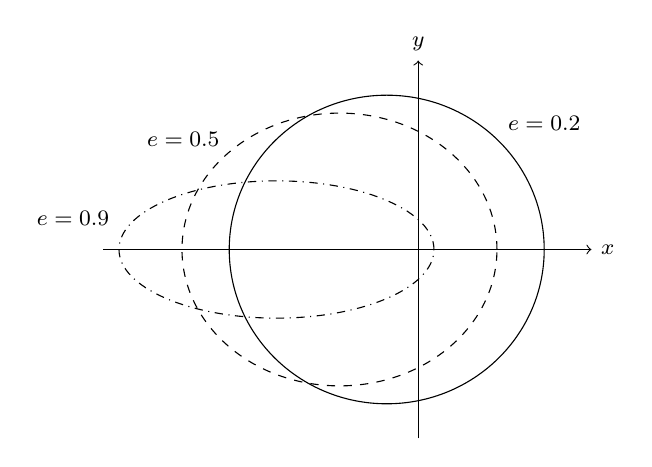
\begin{tikzpicture}[font=\footnotesize,scale=2]
    % Semiasse delle tre ellissi: a=1.
    % e_1=0.2 --> b_1=a*sqrt(1-e_1^2)=0.979796, c_1=a*e_1=0.2.
    % e_2=0.5 --> b_2=a*sqrt(1-e_2^2)=0.866025, c_2=a*e_2=0.5.
    % e_3=0.9 --> b_3=a*sqrt(1-e_3^2)=0.435890, c_3=a*e_3=0.9.
    % Fisso il fuoco nell'origine, quindi i centri si trovano in (-c_i,0).
    \draw [->] (-2,0) -- (1.1,0) node[right] {$x$}; %asse x
    \draw [->] (0,-1.2) -- (0,1.2) node[above] {$y$}; %asse y
    \draw (-0.2,0) ellipse (1 and 0.979796); %ellisse 1
    \draw (0.8,0.8) node {$e=0.2$};
    \draw[dashed] (-0.5,0) ellipse (1 and 0.866025); %ellisse 2
    \draw (-1.2,0.7) node[left] {$e=0.5$};
    \draw[dashdotted] (-0.9,0) ellipse (1 and 0.435890); %ellisse 3
    \draw (-1.9,0.2) node[left] {$e=0.9$};
  \end{tikzpicture}
  \caption[Ellissi con diversi valori di eccentricità]{Ellissi con fuoco comune
    nell'origine del sistema di riferimento, stesso semiasse maggiore $a=1$ ed
    eccentricità differenti}
  \label{fig:ellissi-eccentricita}
\end{figure}

Per la parabola sussistono le seguenti relazioni:
\begin{align}
  c &= a,\\
  p &= 2a,
\end{align}
e per l'iperbole:
\begin{align}
  p &= \frac{b^2}{a} = a(e^2-1), \label{eq:semilato-iperbole}\\
  e &= \sqrt{1+\frac{b^2}{a^2}} =
  \sqrt{1+\frac{p}{a}}, \label{eq:eccentricita-iperbole}\\
  b &= a\sqrt{e^2-1}, \\
  c &= \sqrt{a^2+b^2} = ae.
\end{align}
Osserviamo infine che per tutte le coniche risulta $r(\theta_0\pm\pi/2)=p$.

Inserendo la~\eqref{eq:reciproco-semilato} nella~\eqref{eq:eccentricita-ellisse}
possiamo ricavare l'eccentricità di un'orbita ellittica legata ai parametri
fisici del sistema
\begin{equation}
  \label{eq:eccentricita-orbita-ellisse}
  e = \sqrt{1-\frac{p}{a}} = \sqrt{1-\frac{l_0^2}{GM_\textup{T}\mu^2a}}.
\end{equation}
Si noti che, poiché $l_0\neq 0$ per ipotesi, si ha $0\leq e<1$, coerentemente
con la classificazione illustrata prima. Nel caso di orbita iperbolica dobbiamo
invece utilizzare la~\eqref{eq:eccentricita-iperbole}:
\begin{equation}
  \label{eq:eccentricita-orbita-iperbole}
  e = \sqrt{1+\frac{p}{a}} = \sqrt{1+\frac{l_0^2}{GM_\textup{T}\mu^2a}}
\end{equation}
e qui risulta $e>1$.

L'unica conica chiusa è l'ellisse, quindi abbiamo ricavato la prima legge di
Keplero che per i pianeti del Sistema Solare afferma: \emph{i pianeti,
  considerati puntiformi, descrivono orbite ellittiche di cui il Sole occupa uno
  dei fuochi}.

\subsection{Calcolo della velocità e applicazioni astronomiche}
\label{sec:velocita}
\begin{figure}
  \centering
  \input{Immagini/gnuplot/velocita}
  \caption[Andamento della velocità in funzione dell'anomalia vera]{Andamento
    del modulo quadro della velocità della particella relativa in funzione
    dell'anomalia vera $\chi$ nel caso di orbita ellittica, per diversi valori
    dell'eccentricità $e$. In tutte le curve risulta $a=1$}
  \label{fig:velocita}
\end{figure}
Calcoliamo il modulo quadro della velocità del corpo fittizio di massa ridotta
durante la sua orbita, data dalla~\eqref{eq:velocita-polare}: $v(\theta)^2 =
\norm{\dot{\bm{r}}(\theta)}^2 = \dot{r}^2(\theta) +
r^2(\theta)\dot{\theta}^2$. Ricordando le formule~\eqref{eq:derivata1-r}
e~\eqref{eq:soluzione2-binet} e che $l_0=\mu r^2\dot{\theta}$ abbiamo:
\begin{subequations}
  \begin{align}
    \dot{r}(\theta) &= -\frac{l_0}{\mu}\toder{u}{\theta} = -\frac{l_0}{\mu}
    \left( -\frac{1}{p}e\sin(\theta-\theta_0) \right) = \frac{l_0}{\mu p}e
    \sin(\theta -
    \theta_0), \label{eq:velocita-radiale}\\
    r(\theta)\dot{\theta} &= \frac{l_0}{\mu}u =
    \frac{l_0}{\mu p}(1+e\cos(\theta-\theta_0)). \label{eq:velocita-tangenziale}
  \end{align}
\end{subequations}
Per quanto riguarda il moto ellittico, mettendo insieme le relazioni appena
trovate, la~\eqref{eq:reciproco-semilato} e la~\eqref{eq:orbita} risulta
{\allowdisplaybreaks{\begin{equation}
  \label{eq:velocita-ellisse}
  \begin{split}
    v^2(\theta) &= \dot{r}^2(\theta) + r^2(\theta)\dot{\theta}^2 \\
    &= \left(
      \frac{l_0}{\mu p}
    \right)^2(e^2\sin^2(\theta-\theta_0) + 1 + 2e\cos(\theta-\theta_0) +
    e^2\cos^2(\theta-\theta_0)) \\
    &= \left(
      \frac{l_0}{\mu p}
    \right)^2(1+2e\cos(\theta-\theta_0)+e^2) \\
    &= \left(
      \frac{l_0}{\mu p}
    \right)^2(2(1+e\cos(\theta-\theta_0)) + (e^2-1)) \\
    &= \frac{l_0^2}{\mu^2p}
    \left(
      2\frac{1+e\cos(\theta-\theta_0)}{p} - \frac{1-e^2}{p}
    \right) = \frac{l_0^2}{\mu^2 p}
    \left(
      \frac{2}{r(\theta)} - \frac{1}{a}
    \right) \\
    &= \frac{l_0^2}{\mu^2}\frac{GM_\textup{T}\mu^2}{l_0^2}
    \left(
      \frac{2}{r(\theta)} - \frac{1}{a}
    \right) = GM_\textup{T}
    \left(
      \frac{2}{r(\theta)} - \frac{1}{a}
    \right).
  \end{split}
\end{equation}}
Questa relazione lega il modulo quadro della velocità alla distanza della
particella relativa da $M_\textup{T}$. Si può osservare in particolare che
$v^2(\theta)$ è lineare in $1/r(\theta)$, quindi il modulo della velocità è
massimo quando la particella relativa si trova nel periapside e vale
\begin{equation}
  v^2(\theta_0) = \frac{GM_\textup{T}}{a}\frac{1+e}{1-e}.
\end{equation}
Inoltre il modulo quadro della velocità sarà minimo quando la distanza da
$M_\textup{T}$ è massima, cioè all'apoapside
\begin{equation}
  v^2(\theta_0+\pi) = \frac{GM_\textup{T}}{a}\frac{1-e}{1+e}.
\end{equation}
Questi risultati sono in accordo con la seconda legge di Keplero. L'andamento di
$v^2$ in funzione dell'anomalia vera $\chi$ è riportato nella
Figura~\ref{fig:velocita}.

I calcoli svolti per determinare la velocità nel caso di orbite ellittiche sono
del tutto analoghi a quelli necessari nel caso di orbite paraboliche e
iperboliche, però per le orbite paraboliche $e=1$ quindi
\begin{equation}
  \label{eq:velocita-parabola}
  v^2(\theta) = \frac{2GM_\textup{T}}{r(\theta)},
\end{equation}
mentre per le orbite iperboliche, per le quali il semilato retto e
l'eccentricità sono legati dalla~\eqref{eq:semilato-iperbole}, si ha
\begin{equation}
  \label{eq:velocita-iperbole}
  v^2(\theta) = GM_\textup{T}
    \left(
      \frac{2}{r(\theta)} + \frac{1}{a}
    \right).
\end{equation}

\subsubsection{Velocità nella direzione della linea di vista}
\label{sec:velocita-linea-di-vista}

\begin{figure}[tb]
  \centering
  \input{Immagini/gnuplot/ellisse_vlos}
  \caption[Velocità nella direzione della linea di vista]{Orbita della
    particella relativa nel sistema di riferimento di $M_\textup{T}$. È
    rappresentata la velocità $\bm{v}$ della particella in due punti dell'orbita
    insieme alle componenti radiali, tangenziali e lungo la linea di vista
    $\bm{v}_\textup{los}$. I parametri dell'ellisse sono $e=0.7$ e $a=2$}
  \label{fig:ellisse-vlos}
\end{figure}
Nelle osservazioni astronomiche di un sistema binario, spesso è possibile
misurare solo la componente della velocità dei due corpi lungo la direzione di
vista dell'osservatore. Calcoleremo dapprima la velocità lungo la direzione di
vista $v_\textup{los}$ per la particella relativa, poi riporteremo i risultati
ottenuti ai due corpi. Supponiamo che l'osservatore guardi la particella
relativa nella direzione dell'asse $\versor{x}$, come nella
Figura~\ref{fig:ellisse-vlos}, quindi $v_\textup{los} = \bm{v}\cdot\versor{x}$.
Per semplicità, svolgeremo i calcoli in funzione dell'anomalia vera $\chi$. Per
calcolare $v_\textup{los}$ facciamo le seguenti considerazioni
geometriche. Chiamiamo $\alpha(\chi)$ l'angolo compreso fra la direzione di
$\versor{r}(\chi)$ e del vettore $\dot{\bm{r}}(\chi) \equiv \bm{v}(\chi)$ e sia
per il momento $\chi \in \mathopen{[}0, \pi\mathclose{]}$. La tangente di questo
angolo è data dal rapporto fra la componente tangenziale $r(\chi)\dot{\chi}$
della velocità e la componente radiale $\dot{r}(\chi)$, quindi
\begin{equation}
  \label{eq:angolo-alpha}
  \alpha(\chi) = \arctan\frac{r(\chi)\dot{\chi}}{\dot{r}(\chi)} =
  \arctan\frac{1 + e\cos\chi}{e\sin\chi} = \arctan
  \left(
    \cot\chi + \frac{\csc\chi}{e}
  \right).
\end{equation}
Per $\chi \in \mathopen{]}\pi, 2\pi\mathclose{[}$ dobbiamo prendere qualche
accorgimento. La funzione $\arctan$ ha codominio
$\mathopen{]}-\pi/2, \pi/2\mathclose{[}$, ma nell'intervallo
$\chi \in \mathopen{]}\pi, 2\pi\mathclose{[}$ la componente radiale
$\dot{r}(\chi)$ assume valori negativi, come si può vedere
dalla~\eqref{eq:velocita-radiale} e nella Figura~\ref{fig:ellisse-vlos}, quindi
l'angolo $\alpha(\chi)$ che la velocità forma con la direzione radiale positiva
è maggiore di $\pi/2$. Per ottenere il valore giusto di $\alpha(\chi)$ in questo
intervallo dobbiamo aggiungere $\pi$ al risultato dato
dalla~\eqref{eq:angolo-alpha}, in definitiva
\begin{equation}
  \label{eq:angolo-alpha2}
  \alpha(\chi) =
  \begin{dcases}
    \arctan
    \left(
      \cot\chi + \frac{\csc\chi}{e}
    \right) & \text{se $\chi \in \mathopen{[}0, \pi\mathclose{]}$,}\\
    \arctan
    \left(
      \cot\chi + \frac{\csc\chi}{e}
    \right) + \pi & \text{se $\chi \in \mathopen{]}\pi, 2\pi\mathclose{[}$.}
  \end{dcases}
\end{equation}
Si noti che grazie a questa definizione la funzione $\alpha(\chi)$ è continua
in $\chi = \pi$. Indichiamo con $\beta(\chi)$ l'angolo compreso fra la
direzione del vettore velocità $\bm{v}(\chi)$ e la linea di vista, nel nostro
caso l'asse $\versor{x}$. Poiché $\alpha(\chi)$ è l'angolo fra il verso
positivo della direzione radiale e il vettore $\bm{v}(\chi)$ e la direzione
radiale forma un angolo $\chi$ con la direzione positiva dell'asse
$\versor{x}$, abbiamo $\beta(\chi) = \chi + \alpha(\chi)$ e la componente
della velocità nella direzione della linea di vista è
\begin{figure}[tb]
  \centering
  \input{Immagini/gnuplot/velocita_los}
  \caption[Andamento della velocità nella direzione della di vista in funzione
  dell'anomalia
  vera]{Andamento della velocità lungo la direzione della linea di vista del
    corpo di massa ridotta in funzione dell'anomalia vera nel caso di orbita
    ellittica. Il grafico è stato realizzato per gli stessi valori di
    eccentricità utilizzati nella Figura~\ref{fig:velocita}, con $a=1$}
  \label{fig:velocita-los}
\end{figure}
\begin{equation}
  \begin{split}
    v_\textup{los} &= v(\chi)\cos\beta(\chi) = \sqrt{GM_\textup{T} \left(
      \frac{2}{r(\chi)} - \frac{1}{a}
    \right)}\cos(\chi + \alpha(\chi)) = \\
    &= \sqrt{GM_\textup{T}
    \left(
      \frac{2(1+e\cos\chi)}{a(1-e^2)} - \frac{1}{a}
    \right)}\cos(\chi + \alpha(\chi)).
  \end{split}
\end{equation}
Osserviamo dalla~\eqref{eq:angolo-alpha2} che se $e=0$, cioè per le orbite
circolari, si ha sempre $\alpha(\chi) = \pi/2$, coerentemente col fatto che
per il moto circolare la velocità è sempre tangenziale. Nella
Figura~\ref{fig:velocita-los} è riportato l'andamento di $v_\textup{los}$ in
funzione dell'anomalia $\chi$ per diversi valori dell'eccentricità.

\begin{figure}
  \centering
  \begin{axis}[xlabel=$\theta$,
  ylabel={$v_{\textup{los}}(\theta)$ (\si{\kilo\metre\per\second})},
  legend pos=north west]
  % l'opzione `raw gnuplot' serve per permettere di scrivere uno script
  % gnuplot come argomento di `\addplot'. È una funzione molto comoda ma
  % mal documentata in pgfplots.
  \addplot [raw gnuplot,mark=none,red] gnuplot {
    r(a,e,x)=a*(1-e**2)/(1+e*cos(x));
    GM=5e11;
    v(a,e,x)=sqrt(GM*(2./r(a,e,x)-1/a));
    alpha(x,e)= e==0 ? pi/2 : ((x<=pi) ? atan(1/tan(x)+1/(e*sin(x))) :
                                         atan(1/tan(x)+1/(e*sin(x)))-pi);
    beta(x,e)= e==0 ? x+pi/2 : x+alpha(x,e);
    vlos(a,e,x)=v(a,e,x)*(cos(beta(x,e)));
    a=5e7;
    e=0.5;
    m1=5.0;
    m2=1.0;
    mu=m1*m2/(m1+m2);
    plot [0.001:2*pi] -mu/m1*vlos(a,e,x)-50
  };
  \addplot [raw gnuplot,mark=none,blue] gnuplot {
    r(a,e,x)=a*(1-e**2)/(1+e*cos(x));
    GM=5e11;
    v(a,e,x)=sqrt(GM*(2./r(a,e,x)-1/a));
    alpha(x,e)= e==0 ? pi/2 : ((x<=pi) ? atan(1/tan(x)+1/(e*sin(x))) :
                                         atan(1/tan(x)+1/(e*sin(x)))-pi);
    beta(x,e)= e==0 ? x+pi/2 : x+alpha(x,e);
    vlos(a,e,x)=v(a,e,x)*(cos(beta(x,e)));
    a=5e7;
    e=0.5;
    m1=5.0;
    m2=1.0;
    mu=m1*m2/(m1+m2);
    plot [0.001:2*pi] mu/m2*vlos(a,e,x)-50
  };
  \legend{$m_{1}$,$m_{2}$}
\end{axis}

%%% Local Variables: 
%%% mode: latex
%%% TeX-master: "../../presentazione"
%%% End: 

  \caption[Andamento della velocità dei due corpi nella direzione della di vista
  in funzione dell'anomalia
  vera]{Andamento della velocità dei due corpi lungo la direzione della linea di
    vista in funzione dell'anomalia vera delle loro orbite. Abbiamo posto
    $GM_\textup{T} = \SI{5e11}{\cubic\kilo\metre\per\square\second}$,
    $a = \SI{5e7}{\kilo\metre}$, $e=0.5$ e $m_1/m_2=5$}
  \label{fig:velocita-los-due-corpi}
\end{figure}
Ritorniamo ai due corpi. Per fare questo ci poniamo in un sistema di riferimento
inerziale con origine nella posizione del centro di massa e indichiamo ancora
con $\versor{x}$ la direzione della linea di vista che però non sarà più la
stessa della Figura~\ref{fig:ellisse-vlos}, tuttavia i ragionamenti da
utilizzare sono gli stessi. Osserviamo che $\bm{v}=\dot{\bm{r}}$ e
dalle~\eqref{eq:r1-r2-posizione-relativa-cdm} abbiamo che le velocità dei corpi
di massa $m_1$ e $m_2$ sono, rispettivamente,
$\bm{v}_1 = \bm{v}_\textup{CM}-\mu\bm{v}/m_1$ e
$\bm{v}_2 = \bm{v}_\textup{CM} + \mu\bm{v}/m_2$, quindi le corrispondenti
velocità lungo la direzione della linea di vista sono
$v_{1,\textup{los}} = \bm{v}_1 \cdot \versor{x} = v_\textup{CM,los}-\mu
v_\textup{los}/m_1$
e
$v_{2,\textup{los}} = \bm{v}_2 \cdot \versor{x} = v_\textup{CM,los} + \mu
v_\textup{los}/m_2$.
Le curve che compaiono nella Figura~\ref{fig:velocita-los} sono centrate attorno
allo zero perché avevamo richiesto per ipotesi che il centro di massa fosse a
riposo, ma se il centro di massa si muove con velocità
$\bm{v}_\textup{CM} = v_\textup{CM,los}\versor{x}$ costante nella direzione
$\versor{x}$ della linea di vista, nelle espressioni di $v_{1,\textup{los}}$ e
$v_{2,\textup{los}}$ è presente il termine costante e non nullo
$v_\textup{CM,los}$. Dunque misurando $v_{1,\textup{los}}$ e
$v_{2,\textup{los}}$ in più punti dell'orbita è possibile determinare la
velocità di allontanamento o avvicinamento di un sistema binario rispetto
all'osservatore. Inoltre dalla misura di
$(v_{1,\textup{los}}-v_{textup{CM,los}})/(v_{2,\textup{los}}-v_{textup{CM,los}})$
si ricava il rapporto delle masse dei due corpi $m_2/m_1$. Nota, con altri
metodi che vedremo più avanti, la somma delle due masse è possibile ottenere il
valore delle masse individuali. Nell'esempio della
Figura~\ref{fig:velocita-los-due-corpi} il centro di massa del sistema si sta
allontanando dall'osservatore con velocità $v_\textup{CM,los} =
\SI{-40}{\kilo\metre\per\second}$. Sistemi binari di questo tipo sono chiamati
\emph{binari spettroscopici}.

\subsection{Energia e classificazione energetica delle orbite}
\label{sec:energia-orbite}

Possiamo ora calcolare l'energia meccanica del sistema costituito dai due
corpi. Essa è data dalla somma di due termini: l'energia cinetica $T$ associata
al moto di ciascun corpo e l'energia potenziale gravitazionale $U$. In
definitiva si ha che
\begin{equation}
  \label{eq:energia}
  \begin{split}
    E &= T + U = \frac{1}{2}m_1\dot{\bm{r}}_1^2 + \frac{1}{2}m_2\dot{\bm{r}}_2^2
    - \frac{GM_\textup{T}\mu}{r(\theta)} \\
    &= \frac{1}{2}m_1
    \left(
      -\frac{\mu}{m_1}\dot{\bm{r}}
    \right)^2 + \frac{1}{2}m_2
    \left(
      \frac{\mu}{m_2}\dot{\bm{r}}
    \right)^2 - \frac{GM_\textup{T}\mu}{r(\theta)} \\
    &= \frac{1}{2}\mu v^2(\theta)
    - \frac{GM_\textup{T}\mu}{r(\theta)} = \frac{1}{2}\mu(\dot{r^2(\theta)} +
    r^2(\theta)\dot{\theta}^2) - \frac{GM_\textup{T}\mu}{r(\theta)}.
  \end{split}
\end{equation}
Per le orbite ellittiche, sostituendo nella relazione precedente al posto della
velocità l'espressione data dalla~\eqref{eq:velocita-ellisse} si ha
\begin{equation}
  \label{eq:energia-ellisse}
  E = \frac{1}{2}GM_\textup{T}\mu
  \left(
    \frac{2}{r(\theta)} - \frac{1}{a}
  \right) - \frac{GM_\textup{T}\mu}{r(\theta)} = -\frac{GM_\textup{T}\mu}{2a}.
\end{equation}
Per le orbite paraboliche, usando la~\eqref{eq:velocita-parabola}, si ottiene
\begin{equation}
  E = \frac{1}{2}\frac{2GM_\textup{T}\mu}{r(\theta)} -
  \frac{GM_\textup{T}\mu}{r(\theta)} = 0.
\end{equation}
Infine per le orbite iperboliche, tramite la~\eqref{eq:velocita-iperbole},
ricaviamo
\begin{equation}
    \label{eq:energia-iperbole}
  E = \frac{1}{2}GM_\textup{T}\mu
  \left(
    \frac{2}{r(\theta)} + \frac{1}{a}
  \right) - \frac{GM_\textup{T}\mu}{r(\theta)} = \frac{GM_\textup{T}\mu}{2a}.
\end{equation}
Dunque in tutti i casi l'energia è una costante del moto e dipende solo dalle
masse $m_1$ e $m_2$ dei due corpi (attraverso $M_\textup{T}$ e $\mu$) e dal
semiasse maggiore dell'ellisse descritta dal loro moto relativo, ma non
dall'eccentricità di questa. Naturalmente il fatto che l'energia si conserva non
deve sorprendere perché abbiamo supposto per ipotesi che il sistema fosse
isolato e che l'unica forza agente fosse quella gravitazionale.

Dalla~\eqref{eq:energia} possiamo inoltre osservare che il moto relativo è
equivalente a un moto unidimensionale lungo la direzione radiale e con un
\emph{potenziale efficace}
\begin{figure} %TODO: scegliere valori migliori per il grafico
  \centering
  % coefficienti che compaiono nel potenziale efficace
\pgfmathsetmacro{\a}{25}
\pgfmathsetmacro{\b}{50}
% funzione potenziale efficace
\pgfmathdeclarefunction{ueff}{1}{\pgfmathparse{\a/#1^2-\b/#1}}
%% valori dell'energia
% energia E_0 = minimo di U_eff, il minimo si ha nel punto r = 2a/b e
% U_eff(2a/b) = -b^2/(4a)
\pgfmathsetmacro{\ezero}{-\b^2/(4*\a)}
\pgfmathsetmacro{\euno}{-20} % energia E_1
\pgfmathsetmacro{\edue}{15} % energia E_2

\draw[->] (0,-30) -- (0,30) node[above] {$U_{\textup{eff}}$}; % asse y
\draw[->] (0,0) node[left] {$O$} -- (8,0) node[right] {$r(\theta)$}; %asse x
% grafico della funzione potenziale efficace
\draw[name path=U] [domain=0.4:8,samples=100] plot (\x,{ueff(\x)});
\draw[dashed,name path={E0}] (0,\ezero) node[left] {$E_0$} -- +(8,0);
\draw[dashed,name path={E1}] (0,\euno) node[left] {$E_1$} -- +(8,0);
\draw[dashed] (0,\edue) node[left] {$E_2$} -- +(8,0);
% individuo il punto di intersezione fra il potenziale e l'energia E_0
\path[name intersections={of=U and {E0},by={A}}];
\draw[loosely dashed] (A) -- +(0,-\ezero) node[above] {$r_0$};
% individuo i punti di intersezione fra il potenziale e l'energia E_1
\path[name intersections={of=U and {E1},by={B,C}}];
\draw[loosely dashed] (B) -- +(0,-\euno) node[above] {$r_{\textup{min}}$}
                      (C) -- +(0,-\euno) node[above] {$r_{\textup{max}}$};

%%% Local Variables:
%%% mode: latex
%%% TeX-master: "../../tesi"
%%% End:

  \caption[Andamento del potenziale efficace in funzione della distanza dal
  centro del campo]{Andamento qualitativo del potenziale efficace della
    particella $\mu$ nel problema di Keplero in funzione della distanza dal
    centro del campo. Il grafico rappresenta la funzione $k_1/r^2-k_2/r$, con
    $k_1$ e $k_2$ costanti positive scelte arbitrariamente}
  \label{fig:potenziale-efficace}
\end{figure}
\begin{equation}
  U_\textup{eff}(r(\theta)) = \frac{1}{2}\mu r^2(\theta)\dot{\theta}^2 -
  \frac{GM_\textup{T}\mu}{r(\theta)} = \frac{1}{2}\frac{l_0^2}{\mu r^2(\theta)} -
  \frac{GM_\textup{T}\mu}{r(\theta)}.
\end{equation}
nel quale il termine $l_0/(2\mu r^2(\theta))$ è chiamato \emph{potenziale
  centrifugo}. Nella Figura~\ref{fig:potenziale-efficace} è riportato il grafico
della curva del potenziale efficace. In $r=r_0=l_0/(GM_\textup{T}\mu^2)$ si ha
un punto di minimo per $U_\textup{eff}$ e risulta $U_\textup{eff}(r_0) =
-G^2M_\textup{T}^2\mu^3/(2l_0^2)$. La differenza fra l'energia e
$U_\textup{eff}$ dà $\mu\dot{r}^2/2$, quindi il moto è ammesso solo in quelle
regioni in cui $E-U_\textup{eff}\geq 0$, cioè:
\begin{enumerate}
\item se $E = E_0 = G^2M_\textup{T}^2\mu^3/(2l_0^2)$ risulta $\dot{r}=0$, cioè
  $r(t) = r_0 = \text{costante}$. L'orbita è dunque circolare e il moto
  circolare uniforme con pulsazione $\omega_0 = l_0/(\mu r_0^2)$;
\item se $E = E_1 \in \mathopen{]}E_0,0\mathclose{[}$, il moto è limitato fra le
  distanze apsidali $r_\textup{min}$ e $r_\textup{max}$ e l'orbita è un'ellisse;
\item se $E = E_2 \geq 0$ il moto è limitato inferiormente ma non
  superiormente. Se $E_2 = 0$ l'orbita descritta è una parabola, se $E_2>0$ si
  ha un'iperbole.
\end{enumerate}

Inserendo la~\eqref{eq:energia-ellisse}
nella~\eqref{eq:eccentricita-orbita-ellisse} e la~\eqref{eq:energia-iperbole}
nella~\eqref{eq:eccentricita-orbita-iperbole} abbiamo che sia per orbite
ellittiche sia per orbite iperboliche sussiste la seguente relazione fra energia
ed eccentricità dell'orbita
\begin{equation}
  \label{eq:eccentricita-energia}
  e = \sqrt{1+\frac{2El_0^2}{G^2M_\textup{T}^2\mu^3}}.
\end{equation}
Si noti che questa relazione è valida anche per le orbite paraboliche perché in
questo caso l'energia è nulla e l'eccentricità vale $1$.

Il corpo fittizio $M_\textup{T}$ esercita un'attrazione sulla particella
relativa, tuttavia la presenza del potenziale centrifugo non
nullo\footnote{Si ricordi che abbiamo supposto per ipotesi che sia $l_0\neq 0$.}
impedisce che questa possa cadere nel centro della forza se il campo generato è
quello gravitazionale. Infatti abbiamo
\begin{equation}
  0\leq \frac{1}{2}\mu\dot{r}^2 = E - U_\textup{eff}(r) = E -
  \frac{1}{2}\frac{l_0^2}{\mu r^2} - \frac{GM_\textup{T}\mu}{r}
\end{equation}
che può essere riscritta come
\begin{equation}
  \frac{1}{2}\frac{l_0^2}{\mu} + GM_\textup{T}\mu r \leq Er^2
\end{equation}
e facendo il limite per $r \to 0$ abbiamo
\begin{equation}
  \frac{1}{2}\frac{l_0^2}{\mu} \leq 0,
\end{equation}
ma questo non è possibile poiché tutte le variabili che compaiono al primo
membro sono definite positive.

Prendiamo in considerazione il caso delle orbite
ellittiche. Dall'espressione~\eqref{eq:velocita-areolare} della velocità
areolare della particella relativa abbiamo
\begin{equation}
  l_0 \dd t = 2\mu\dd A.
\end{equation}
L'area di un'ellisse di semiassi maggiore e minore rispettivamente $a$ e $b$ è
pari a $\pi ab$ quindi integrando l'equazione precedente in un intero periodo
ricaviamo
\begin{equation}
    \int_{t_0}^{t_0+P} l_0\dd t = Pl_0 = 2\mu\pi ab.
\end{equation}
Dal valore~\eqref{eq:energia-ellisse} dell'energia del sistema nel caso di
orbite ellittiche abbiamo
\begin{equation}
  a = \frac{GM_\textup{T}\mu}{2\abs{E}},
\end{equation}
dunque, ricordando le~\eqref{eq:semiasse-minore-ellisse}
e~\eqref{eq:eccentricita-energia}, il quadrato del periodo di rivoluzione è
\begin{equation}
  \label{eq:terza-legge-keplero}
  \begin{split}
    P^2 &= \frac{4\pi^2\mu^2a^2b^2}{l_0^2} = \frac{4\pi^2\mu^2a^4(1-e^2)}{l_0^2}
    = \frac{4\pi^2\mu^2a^4}{l_0^2}\frac{2\abs{E}l_0^2}{G^2M_\textup{T}^2\mu^3} \\
    &= 4\pi^2a^4\frac{1}{aGM_\textup{T}} = \frac{4\pi^2a^3}{GM_\textup{T}}.
  \end{split}
\end{equation}
Questa equazione esprime la terza legge di Keplero: \emph{il quadrato del
  periodo di rivoluzione di un pianeta è proporzionale al cubo del semiasse
  maggiore dell'orbita}.

\subsubsection{Variazioni dell'energia}
\label{sec:variazioni energia}

Vogliamo ora vedere come varia il semiasse maggiore di un'orbita ellittica della
particella di massa ridotta in funzione dell'energia. Per fare ciò differenziamo
la~\eqref{eq:energia-ellisse} rispetto ad $a$
\begin{equation}
  \dd E = \frac{GM_\textup{T}\mu}{2a^2}\dd a.
\end{equation}
Osserviamo che $\dd E$ e $\dd a$ hanno lo stesso segno, quindi se l'energia
aumenta aumenterà anche il semiasse maggiore, se l'energia diminuisce lo stesso
farà $a$. Questo risultato ha importanti conseguenze astronomiche. Se un sistema
binario di corpi celesti perde energia, cioè l'energia diventa ancora più
negativa, il semiasse maggiore diminuirà rendendo il sistema più legato; al
contrario, se il sistema acquista energia, cioè questa diventa meno negativa, il
semiasse maggiore aumenterà e il sistema diventerà meno legato. Al limite, se
l'energia diventa nulla o positiva il sistema non sarà più legato.

Consideriamo ora il caso in cui il sistema sta perdendo energia a causa della
diminuzione della massa di uno dei corpi, per esempio
$m_1$.\footnote{Per un'applicazione si può consultare
  \textcite{padmanabhan:stars}.}
Supponiamo che i due corpi descrivano orbite ellittiche e indichiamo la
variazione della massa di $m_1$ con $\Delta M = m_1 - m_\textup{R}$, dove
$m_\textup{R}$ è la massa residua del corpo. Facciamo l'ipotesi semplificatrice,
ma non del tutto corretta, che dopo la perdita di massa da parte di $m_1$ la
velocità
\begin{equation}
  v^2(\theta) = G(m_1 + m_2)
  \left(
    \frac{2}{r(\theta)} - \frac{1}{a}
  \right)
\end{equation}
resti invariata, così come il semiasse maggiore $a$ dell'orbita. In questo modo,
ponendo $M'_\textup{T}=m_\textup{R}+m_2$ e $\mu' = m_\textup{R}m_2/(m_\textup{R}
+ m_2)$, l'energia finale del sistema sarà
\begin{equation}
  \begin{split}
    E' &= \frac{1}{2}\mu'v^2 - \frac{GM'_\textup{T}\mu'}{r(\theta)} \\
    &= \frac{1}{2}\frac{m_\textup{R}m_2}{m_\textup{R} + m_2}G(m_1 + m_2)
    \left(
      \frac{2}{r(\theta)} - \frac{1}{a}
    \right) - G\frac{m_\textup{R}m_2}{r(\theta)} \\
    &= Gm_\textup{R}m_2
    \left(
      \frac{m_1 + m_2}{2(m_\textup{R} + m_2)}
      \left(
        \frac{2}{r(\theta)} - \frac{1}{a}
      \right) - \frac{1}{r(\theta)}
    \right).
  \end{split}
\end{equation}
Affinché il sistema rimanga legato anche dopo la perdita di massa del corpo
$m_1$ deve risultare ancora $E' < 0$, invece il sistema si distruggerà se $E'
\geq 0$, cioè
\begin{equation}
  \begin{split}
    0 &\leq \frac{m_1 + m_2}{2(m_\textup{R} + m_2)}
    \left(
      \frac{2}{r(\theta)} - \frac{1}{a}
    \right) - \frac{1}{r(\theta)} \\
    &= \frac{1}{r(\theta)}
    \left(
      \frac{m_1 + m_2}{m_\textup{R} + m_2} - 1
    \right) - \frac{m_1 + m_2}{2a(m_\textup{R} + m_2)} \\
    &= \frac{1}{r(\theta)}\frac{m_1 + m_2 - m_\textup{R} - m_2}{m_\textup{R} +
      m_2} - \frac{m_1 + m_2}{2a(m_\textup{R} + m_2)} \\
    &= \frac{1}{r(\theta)}\frac{\Delta M}{m_\textup{R} +
      m_2} - \frac{m_1 + m_2}{2a(m_\textup{R} + m_2)},
  \end{split}
\end{equation}
da cui
\begin{equation}
  \Delta M \geq \frac{1}{2}\frac{r(\theta)}{a}(m_1 + m_2).
\end{equation}
Per stimare il valore minimo di $\Delta M$ per il quale il sistema si distrugge,
scegliamo di valutare $r(\theta)$ al periapside, cioè in $\theta = \theta_0$,
perché il sistema è maggiormente legato in questo punto, pertanto
\begin{equation}
    \Delta M \geq \frac{1}{2}\frac{r(\theta_0)}{a}(m_1 + m_2) =
    \frac{1}{2}(1 - e)(m_1 + m_2).
\end{equation}
Da questa relazione possiamo dedurre che all'aumentare dell'eccentricità
iniziale $e$, diventa necessaria una minor quantità di massa persa da parte del
corpo $m_1$ affinché il sistema non sia più stabile. Inoltre nel caso di orbite
originali circolari, cioè $e=0$, e $m_1 \neq m_2$ il sistema non potrà
distruggersi se il corpo che perde massa è il più piccolo dei due, perché non
può essere soddisfatta la condizione $\Delta M \geq (m_1 + m_2)/2$.

\section{Formalismo lagrangiano e hamiltoniano}
\label{sec:formalismo-lagrange}

\subsection{Introduzione alla meccanica lagrangiana e hamiltoniana}
\label{sec:intro-lagrange}

La meccanica newtoniana descrive l'evoluzione di un sistema fisico attraverso la
\emph{seconda legge del moto di Newton}. Nella seconda metà del diciottesimo
secolo il fisico e matematico francese di origine italiana Joseph-Louis Lagrange
propose una formulazione alternativa della meccanica che ora presentiamo
brevemente.

Un sistema fisico composto da $N$ particelle è descritto nello spazio da $3N$
coordinate, ma se il sistema è soggetto a dei vincoli queste $3N$ grandezze
potrebbero essere fra loro legate. Se i vincoli sono olonomi\footnote{Un vincolo
  si dice \emph{olònomo} se è esprimibile sotto forma di un'equazione del tipo
  $f(\bm{r}_1,\dots,\bm{r}_N,t)=0$, dove le $\bm{r}_i$ rappresentano le
  posizioni delle $N$ particelle all'istante $t$.} ed espressi da $k$ equazioni,
allora è possibile introdurre $n=3N-k$ coordinate indipendenti che indichiamo
con $q_1,\dots,q_n$ e che determinano univocamente il sistema tenendo conto dei
vincoli. Le $q_i$ sono dette \emph{coordinate generalizzate} o
\emph{lagrangiane}, non hanno necessariamente le dimensioni di una lunghezza e
la loro scelta non è univoca; $n$, il numero di grandezze indipendenti, è
chiamato \emph{numero di gradi di libertà}. D'ora in poi indicheremo per brevità
con $\bm{q} = (q_1,\dots,q_n)$ l'insieme delle $n$ coordinate generalizzate e
con $\dot{\bm{q}} = (\dot{q}_1,\dots,\dot{q}_n)$ l'insieme delle \emph{velocità
  generalizzate} sebbene, come già osservato, a rigore non è detto che tutte
queste grandezze abbiano la stessa dimensione fisica. Definiamo la
\emph{funzione di Lagrange} o \emph{lagrangiana}
$\mathcal{L}(\bm{q},\dot{\bm{q}},t)$
\begin{equation}
  \mathcal{L}(\bm{q},\dot{\bm{q}},t) = T(\bm{q},\dot{\bm{q}},t) -
  U(\bm{q},\dot{\bm{q}},t)
\end{equation}
dove $T(\bm{q},\dot{\bm{q}},t)$ è l'\emph{energia cinetica} del sistema e
$U(\bm{q},\dot{\bm{q}},t)$ è l'energia potenziale, chiamata \emph{potenziale
  generalizzato} quando dipende dalle velocità $\dot{\bm{q}}$. Nella meccanica
lagrangiana l'evoluzione del sistema è descritto dalle $n$ equazioni
differenziali del secondo ordine chiamate \emph{equazioni di Lagrange}
\begin{equation}
  \label{eq:lagrange}
  \toder{}{t}
  \left(
    \parder{\mathcal{L}}{\dot{q}_i}
  \right) = \parder{\mathcal{L}}{q_i} \qquad (i=1,2,\dots,n).
\end{equation}
La grandezza
\begin{equation}
  p_i = \parder{\mathcal{L}}{\dot{q}_i}
\end{equation}
è chiamata \emph{momento coniugato} alla variabile generalizzata $q_i$.
Dalla~\eqref{eq:lagrange} si vede subito che, se la lagrangiana non dipende
esplicitamente dalla coordinata generalizzata $q_i$, il corrispondente momento
coniugato è una costante del moto. In questo caso la $q_i$ si dice
\emph{ciclica}.

Nella prima metà del 1800 il fisico e matematico irlandese William Rowan
Hamilton riformulò la meccanica lagrangiana. Nel formalismo lagrangiano le
variabili fondamentali sono le coordinate generalizzate $\bm{q}$ che
costituiscono lo \emph{spazio delle configurazioni}, invece nel formalismo
hamiltoniano si passa alle \emph{variabili canoniche} $(\bm{q},\bm{p})$ che
formano lo \emph{spazio delle fasi}. La \emph{funzione di Hamilton} o
\emph{hamiltoniana} è la funzione definita dalla seguente trasformazione di
Legendre della lagrangiana
\begin{equation}
  \mathcal{H}(\bm{q},\bm{p},t) = \sum_{i=1}^n\dot{q}_ip_i -
  \mathcal{L}(\bm{q},\dot{\bm{q}},t).
\end{equation}
In alcuni contesti l'hamiltoniana è chiamata anche \emph{funzione energia}. Nel
caso in cui l'energia cinetica è una funzione omogenea di secondo grado delle
velocità generalizzate $\dot{q}_i$ e il potenziale non dipende da esse,
l'hamiltoniana coincide con l'energia meccanica totale del sistema $E = T +
U$. Se inoltre l'hamiltoniana non dipende esplicitamente dal tempo, l'energia
del sistema è un integrale primo del moto. Le equazioni del moto in questo
formalismo sono date dalle seguenti $2n$, per $i=1,2,\dots,n$, equazioni
differenziali del primo ordine, chiamate \emph{equazioni di Hamilton}
\begin{subequations}
  \begin{align}
    \parder{\mathcal{H}}{p_i} &= \dot{q}_i, \\
    \parder{\mathcal{H}}{q_i} &= -\dot{p}_i.
  \end{align}
\end{subequations}

Maggiori dettagli su questi formalismi possono essere trovati in qualsiasi libro
di meccanica classica come \textcites{goldstein:meccanica}{landau:meccanica}.

\subsection{Risoluzione del problema dei due corpi}
\label{sec:risoluzione-lagrange}

Consideriamo il sistema costituito dai due corpi puntiformi della
Figura~\ref{fig:due-corpi}. Come fatto nel paragrafo~\ref{sec:formalismo-newton}
introduciamo anche i vettori posizione relativa e posizione del centro di massa
dati rispettivamente dalla~\eqref{eq:posizione-relativa} e
dalla~\eqref{eq:centro-di-massa} e quindi i vettori di posizione sono legati a
questi dalle relazioni~\eqref{eq:r1-r2-posizione-relativa-cdm}. Le quantità di
moto dei due corpi che costituiscono il sistema sono
\begin{subequations}
  \begin{align}
    \bm{p}_1 &= \toder{m_1\bm{r}_1}{t} = m_1\dot{\bm{r}}_1, \\
    \bm{p}_2 &= \toder{m_2\bm{r}_2}{t} = m_2\dot{\bm{r}}_2
  \end{align}
\end{subequations}
Supponiamo che le forze con cui interagiscono i due corpi derivino da un unico
potenziale $U=U(\bm{r})$ dipendente solo dalla posizione relativa fra i due
corpi, dunque la lagrangiana del sistema è data da
\begin{equation}
  \label{eq:lagrangiana-due-corpi}
  \begin{split}
    \mathcal{L} &= T - U = \frac{1}{2}m_1\dot{\bm{r}}_1^2 +
    \frac{1}{2}m_2\dot{\bm{r}}_2^2 - U(\bm{r}) \\
    &= \frac{1}{2}m_1
    \left(
      \dot{\bm{r}}_\textup{CM} -
      \frac{\mu}{m_1}\dot{\bm{r}}
    \right)^2 + \frac{1}{2}m_2
    \left(
      \dot{\bm{r}}_\textup{CM} +
      \frac{\mu}{m_2}\dot{\bm{r}}
    \right)^2 - U(\bm{r}) \\
    &= \frac{1}{2}M_\textup{T}\dot{\bm{r}}_\textup{CM}^2 +
    \frac{1}{2}\mu\dot{\bm{r}}^2 - U(\bm{r}),
\end{split}
\end{equation}
dove $M_\textup{T}=m_1+m_2$ e $\mu=m_1m_2/(m_1+m_2)$ sono, rispettivamente, la
massa totale e la massa ridotta già introdotte nel
paragrafo~\ref{sec:formalismo-newton}. I momenti coniugati alle coordinate
$\bm{r}_\textup{CM}$ e $\bm{r}$ sono
\begin{subequations}
  \begin{align}
    \bm{p}_\textup{CM} &= \parder{\mathcal{L}}{\dot{\bm{r}}_\textup{CM}} =
    M_\textup{T}\dot{\bm{r}}_\textup{CM} = m_1\dot{\bm{r}}_1+m_2\dot{\bm{r}}_2 =
    \bm{p}_1 + \bm{p}_2, \\
    \bm{p} &= \parder{\mathcal{L}}{\dot{\bm{r}}} = \mu\dot{\bm{r}} =
    \frac{m_2\bm{p}_1 + m_1\bm{p}_2}{m_1 + m_2}. \label{eq:momento-relativo}
  \end{align}
\end{subequations}
dove $\bm{p}_\textup{CM}$ è il \emph{momento totale} e $\bm{p}$ il \emph{momento
  relativo}. Osserviamo infine che
\begin{equation}
  \frac{\bm{p}}{\mu} = \frac{\bm{p}_1}{m_1} + \frac{\bm{p}_2}{m_2}.
\end{equation}
Poiché la coordinata $\bm{r}_\textup{CM}$ è ciclica nella
lagrangiana~\eqref{eq:lagrangiana-due-corpi}, il momento totale
$\bm{p}_\textup{CM}=M_\textup{T}\dot{\bm{r}}_\textup{CM}$ è una costante del
moto: il centro di massa si muove di moto rettilineo uniforme oppure è in
quiete. Scegliamo come nostro sistema di riferimento uno in cui il centro di
massa è in quiete, cioè $\dot{\bm{r}}_\textup{CM} = \bm{0}$, di modo che la
lagrangiana diventa
\begin{equation}
  \label{eq:lagrangiana2-due-corpi}
  \mathcal{L} = \frac{1}{2}\mu\dot{\bm{r}}^2 - U(\bm{r}).
\end{equation}
Il primo termine di questa lagrangiana è l'energia cinetica di un corpo fittizio
di massa $\mu$ e posizione $\bm{r}$ rispetto all'origine del sistema di
riferimento. Il vettore $\bm{r}$ svolge dunque il ruolo di coordinate
generalizzate e il numero di grandezze indipendenti che lo individuano è uguale
al numero di gradi di libertà del sistema.  L'equazione di Lagrange per la
coordinata $\bm{r}$ è
\begin{equation}
  \toder{\bm{p}}{t} = -\toder{U(\bm{r})}{\bm{r}} \iff \mu\toder[2]{\bm{r}}{t} =
  -\nabla U(\bm{r}),
\end{equation}
che è equivalente alla~\eqref{eq:f21-mu} ricordando che $\bm{F}_{21} =
-\nabla U(\bm{r})$, perché abbiamo supposto che le forze agenti nel sistema
derivino dall'unico potenziale $U$.

L'energia cinetica $T$ è una funzione omogenea di secondo grado della velocità
generalizzata $\dot{\bm{r}}$, mentre l'energia potenziale $U$ non dipende da
essa, quindi l'hamiltoniana del sistema
\begin{equation}
  \mathcal{H} = \bm{p}\cdot\dot{\bm{r}} - \mathcal{L} = \frac{\bm{p}^2}{2\mu} +
  U(\bm{r})
\end{equation}
rappresenta esattamente l'energia meccanica totale. L'hamiltoniana non dipende
esplicitamente dal tempo, pertanto l'energia del sistema è una costante del
moto. Le equazioni di Hamilton per le variabili canoniche $(\bm{r},\bm{p})$ sono
\begin{subequations}
  \begin{align}
    \parder{\mathcal{H}}{\bm{p}} &= \dot{\bm{r}} \iff \frac{\bm{p}}{\mu} =
    \dot{\bm{r}}, \\
    \parder{\mathcal{H}}{\bm{r}} &= -\dot{\bm{p}} \iff \toder{\bm{p}}{t} =
    -\toder{U(\bm{r})}{\bm{r}} = -\nabla U(\bm{r}).
  \end{align}
\end{subequations}
La prima equazione di Hamilton è equivalente alla~\eqref{eq:momento-relativo},
mentre la seconda è equivalente alla~\eqref{eq:f21-mu}.

Supponiamo ora che il potenziale dipenda in particolare dalla distanza $r$ fra i
due corpi e non dalla direzione del vettore $\bm{r}$, cioè $U=U(r)$. Questo
comporta, per l'equazione di Lagrange o per la seconda equazione di Hamilton,
che la forza che agisce sulla particella relativa è centrale, quindi, come
abbiamo visto nel paragrafo~\ref{sec:problema-keplero}, il vettore momento
angolare $\bm{l}_0$ è un integrale primo e il moto si svolge in un piano. Allora
il sistema ha due gradi di libertà e possiamo riscrivere la
lagrangiana~\eqref{eq:lagrangiana2-due-corpi} nelle coordinate generalizzate
polari $r,\theta$
\begin{equation}
  \mathcal{L} = \frac{1}{2}\mu(\dot{r}^2+r^2\dot{\theta}^2) - U(r).
\end{equation}
La coordinata $\theta$ è ciclica e quindi il suo momento coniugato
\begin{equation}
  p_\theta = \parder{\mathcal{L}}{\dot{\theta}} = \mu r^2\dot{\theta} = l_0
\end{equation}
è una costante del moto. Abbiamo così trovato nuovamente che il modulo del
vettore momento angolare è costante e, ricordando il risultato del
paragrafo~\ref{sec:problema-keplero}, siamo stati in grado di dimostrare la
validità della seconda legge di Keplero. L'equazione di Lagrange per la
coordinata $r$ è
\begin{equation}
  \label{eq:eq-lagrange-due-corpi}
  \mu\ddot{r} = \mu r\dot{\theta}^2 - \parder{U(r)}{r}.
\end{equation}
Se il potenziale è quello di attrazione gravitazionale fra la particella
relativa e $M_\textup{T}$, cioè
\begin{equation}
  \label{eq:potenziale-gravitazionale}
  U(r) = -\frac{GM_\textup{T}\mu}{r},
\end{equation}
allora l'equazione di Lagrange~\eqref{eq:eq-lagrange-due-corpi} diventa
l'equazione del moto~\eqref{eq:forza-mu-radiale} e si può ricavare l'equazione
dell'orbita~\eqref{eq:orbita} nello stesso modo. Il momento coniugato alla
coordinata $r$ è
\begin{equation}
  p = \parder{\mathcal{L}}{\dot{r}} = \mu\dot{r}
\end{equation}
e pertanto l'hamiltoniana in coordinate polari e con il potenziale
gravitazionale~\eqref{eq:potenziale-gravitazionale} è data da
\begin{equation}
  \begin{split}
    \mathcal{H} &= p\dot{r} + p_\theta\dot{\theta} - \mathcal{L} =
    \frac{1}{2}\mu(\dot{r}^2+r^2\dot{\theta}^2) - \frac{GM_\textup{T}\mu}{r} \\
    &= \frac{1}{2}\mu\dot{r}^2 + \frac{1}{2}\frac{l_0^2}{\mu r^2} -
    \frac{GM_\textup{T}\mu}{r},
  \end{split}
\end{equation}
che è equivalente all'espressione dell'energia data nella~\eqref{eq:energia}.

Naturalmente usando il formalismo lagrangiano e hamiltoniano siamo giunti agli
stessi risultati trovati con il formalismo newtoniano.

\section{Soluzione del problema di Keplero}
\label{sec:soluzione-problema}

Nel paragrafo~\ref{sec:equazione-dellorbita} abbiamo ricavato
l'equazione~\eqref{eq:orbita} dell'orbita della particella di massa ridotta per
il problema di Keplero e nel paragrafo~\ref{chap:due-corpi} abbiamo visto che
i vettori posizione $\bm{r}_1$ e $\bm{r}_2$, nel sistema di riferimento del
centro di massa, delle particelle di massa rispettivamente $m_1$ e $m_2$ sono
legati al vettore $\bm{r}$, che individua la posizione della particella
relativa, dalle relazioni~\eqref{eq:r1-r2-nel-cdm}. Allora sostituendo
la~\eqref{eq:orbita} nelle~\eqref{eq:r1-r2-nel-cdm} troviamo che le orbite dei
due corpi nel sistema di riferimento del centro di massa sono
\begin{figure}
  \centering
  % a=1, e=0.8, b=a*sqrt(1-e^2)=0.6, c=a*e=0.8, p=a*(1-e^2)=0.36,
  % m_1 = 5, m_2=1, mu=m_1*m_2/(m_1+m_2)=0.8333,
  % a_1=a*mu/m_1=0.1667, b_1=b*mu/m_1=0.1, c=a_1*e=0.1333
  % a_2=a*mu/m_2=0.8333, b_1=b*mu/m_2=0.5, c=a_2*e=0.6667
  \begin{tikzpicture}[font=\footnotesize,scale=2.5]
    \draw[->] (-1.6,0) -- (0.4,0) node[right] {$x$}; %asse x
    \draw[->] (0,-0.7) -- (0,0.7) node[above] {$y$}; %asse y
    \draw (0.1333,0) ellipse (0.1667 and 0.1); %ellisse di m_1
    \node at (0.35,0.1) {$m_1$};
    \draw[dashed] (-0.6667,0) ellipse (0.8333 and 0.5); %ellisse di m_2
    \node at (-1.2,0.5) {$m_2$};
  \end{tikzpicture}
  \quad
  \begin{tikzpicture}[font=\footnotesize,scale=2.5]
    \draw[->] (-1.9,0) -- (0.3,0) node[right] {$x$}; %asse x
    \draw[->] (0,-0.7) -- (0,0.7) node[above] {$y$}; %asse y
    \draw (-0.8,0) ellipse (1 and 0.6); %ellisse della particella ridotta
    \node [below left] at (0,0) {$m_1$};
    \node at (-1.6,0.5) {$\mu$};
  \end{tikzpicture}
  % \input{Immagini/gnuplot/orbite_ellittiche}
  \caption[Soluzione del problema di Keplero]{Nella figura di sinistra sono
    riportate le orbite ellittiche dei due corpi nel sistema di riferimento del
    centro di massa. Nella figura di destra è rappresentata l'orbita della
    particella relativa nel sistema di riferimento con origine nel corpo di
    massa $m_1$. Abbiamo posto $m_1=5$ e $m_2=1$ in unità arbitrarie, i
    parametri delle ellissi sono $a=1$ ed $e=0.8$}
  \label{fig:orbite-ellittiche}
\end{figure}
\begin{subequations}
  \begin{align}
    r_1(\theta) &= -\frac{\mu}{m_1}r(\theta) =
    -\frac{\mu}{m_1}\frac{p}{1+e\cos(\theta - \theta_0)},\\
    r_2(\theta) &= \frac{\mu}{m_2}r(\theta) =
    \frac{\mu}{m_2}\frac{p}{1+e\cos(\theta - \theta_0)}.
  \end{align}
\end{subequations}
Nella Figura~\ref{fig:orbite-ellittiche} mostriamo le orbite dei due corpi e del
corpo di massa ridotta nel caso di orbite ellittiche. Come si può osservare,
entrambi i corpi ruotano intorno al centro di massa ma mentre il corpo più
massivo, nell'esempio in figura $m_1$, rimane vicino a questo, il corpo meno
massivo descrive orbite più larghe. Dalle
relazioni~\eqref{eq:r1-r2-posizione-relativa-cdm} si vede inoltre che il centro
di massa giace sempre sulla congiungente $\bm{r}$ dei due corpi, quindi $m_1$ e
$m_2$ sono sempre opposti rispetto al centro di massa durante il loro moto
orbitale.

\subsection{Integrali primi del moto}
\label{sec:integrali-primi}

Si dimostra che in un sistema isolato, come quello composto dai due corpi, con
$n$ gradi di libertà esistono $2n+1$ integrali primi del moto indipendenti (si
veda \textcite{landau:meccanica}). Abbiamo visto che il problema di Keplero ha
due gradi di libertà e finora abbiamo trovati quattro costanti: l'energia $E$
del sistema e le tre componenti del vettore momento angolare $\bm{l}_0$. Per
tutti i campi centrali con forza del tipo $\bm{F} = -k/r^2\versor{r}$, agente su
un corpo di massa $\mu$, esiste un altro vettore costante chiamato
\emph{vettore di Laplace-Runge-Lenz} e definito da
\begin{equation}
  \bm{A} = \bm{p}\times\bm{l}_0 - \mu k\versor{r}.
\end{equation}
Per il campo gravitazionale abbiamo $k=GM_\textup{T}\mu$, dove $M_\textup{T}$ è
la massa del corpo che genera il campo. Verifichiamo che il vettore $\bm{A}$ è
una costante del moto
\begin{equation}
  \begin{split}
    \toder{\bm{A}}{t} &= \dot{\bm{p}}\times\bm{l}_0 + \bm{p}\times\dot{\bm{l}_0}
    - \mu k\toder{\versor{r}}{t} = \bm{F}\times\bm{l}_0 - \mu
    k\dot{\theta}\versor{\theta} \\
    &= -\frac{k}{r^2}\versor{r}\times \mu r^2\dot{\theta}\versor{z} -
    \mu k\dot{\theta}\versor{\theta} = \mu k\dot{\theta}\versor{\theta} -
    \mu k\dot{\theta}\versor{\theta} = \bm{0}.
  \end{split}
\end{equation}
I vettori $\bm{A}$ e $\bm{l}_0$ sono perpendicolari, infatti
$\bm{A}\cdot\bm{l}_0 = (\bm{p}\times\bm{l}_0)\cdot\bm{l}_0 - (\mu
k\versor{r})\cdot\bm{l}_0 = 0$.
Dunque da ciò deriva che $\bm{A}$ giace nel piano orbitale. Questo vettore
permette inoltre di ricavare facilmente l'equazione dell'orbita, infatti
indicando con $\theta$ l'angolo fra il vettore posizione $\bm{r}$ e la direzione
fissa del vettore $\bm{A}$ abbiamo
$\bm{A}\cdot\bm{r} = Ar\cos\theta = \bm{r}\cdot(\bm{p}\times\bm{l}_0) - \mu kr =
\bm{l}_0\cdot(\bm{r}\times\bm{p}) - \mu kr$, da cui
\begin{equation}
  \frac{1}{r} = \frac{\mu k}{l_0^2}
  \left(
    1 + \frac{A}{\mu k}\cos\theta
  \right).
\end{equation}
Confrontando questa equazione con la~\eqref{eq:soluzione2-binet} notiamo che
$\bm{A}$ è diretto parallelamente al vettore $\bm{r}$ nel punto di periapside e
che ha modulo $A = \mu ke$.

Adesso conosciamo sette costanti del moto, ma non sono tutte fra loro
indipendenti. Un prima relazione che lega queste costanti è l'ortogonalità fra
$\bm{A}$ e $\bm{l}_0$, l'altra deriva da $A = \mu ke$, dove l'eccentricità $e$ è
data dalla~\eqref{eq:eccentricita-energia}, quindi $A^2 = \mu^2k^2e^2 = \mu^2k^2
+ 2\mu El_0^2$. Questo prova l'esistenza di cinque costanti indipendenti fra le
sette complessivamente trovate.

\section{Geometria del sistema binario}
\label{sec:geometria-sistema}

% TODO: mettere figure e relativi riferimenti
In questo paragrafo ci proponiamo di determinare come un osservatore vede un
sistema binario nel proprio cielo. Per fare ciò consideriamo il sistema di
riferimento destrorso $Ox'y'z'$ intrinseco al sistema binario, cioè con origine
nel fuoco dell'orbita, assi $x'$ e $y'$ complanari al piano dell'orbita e $z'$
ortogonale a questo. Gli assi $x'$ e $y'$ sono diretti, rispettivamente, come
gli assi $x$ e $y$ della figura~\ref{fig:ellisse}, con $x'$ diretto verso il
periapside. Consideriamo ora il sistema di riferimento ausiliario $Oxyz$,
ottenuto ruotando attorno all'asse $z\equiv z'$ il sistema $Ox'y'z'$ di un
angolo $\phi_0$. Le coordinate nel sistema di riferimento ausiliario possono
essere ottenute da quelle del sistema di riferimento intrinseco con la seguente
trasformazione scritta in forma matriciale (si
veda~\textcite{goldstein:meccanica})
\begin{equation}
  \begin{pmatrix}
    x \\
    y \\
    z \\
  \end{pmatrix} =
  \begin{pmatrix}
    \cos\phi_0 & -\sin\phi_0 & 0 \\
    \sin\phi_0 & \cos\phi_0  & 0 \\
    0          & 0           & 1
  \end{pmatrix}
  \begin{pmatrix}
    x' \\
    y' \\
    z'
  \end{pmatrix}.
\end{equation}
Supponiamo ora che un osservatore, posto a distanza $D$ dal sistema, si trovi
nel piano $xz$ e guardi il piano dell'orbita lungo un asse $x''$ che forma un
angolo $i$, che prende il nome di \emph{angolo di inclinazione}, con la
direzione dell'asse $z\equiv z'$. Consideriamo dunque un nuovo sistema di
riferimento destrorso $Ox''y''z''$, ottenuto ruotando attorno all'asse
$y''\equiv y$ il sistema $Oxyz$ di un angolo $\pi/2 - i$. La trasformazione che
permette di passare dal sistema di riferimento ausiliario a questo nuovo sistema
è la seguente
\begin{equation}
  \begin{pmatrix}
    x'' \\
    y'' \\
    z''
  \end{pmatrix} =
  \begin{pmatrix}
    \sin i  & 0 & \cos i \\
    0       & 1 & 0      \\
    -\cos i & 0 & \sin i
  \end{pmatrix}
  \begin{pmatrix}
    x \\
    y \\
    z
  \end{pmatrix}.
\end{equation}
Possiamo passare direttamente dal sistema di riferimento intrinseco al piano del
cielo combinando le due trasformazioni
\begin{equation}
  \begin{split}
    \begin{pmatrix}
      x'' \\
      y'' \\
      z''
    \end{pmatrix} &=
    \begin{pmatrix}
      \sin i  & 0 & \cos i \\
      0       & 1 & 0      \\
      -\cos i & 0 & \sin i
    \end{pmatrix}
    \begin{pmatrix}
      \cos\phi_0 & -\sin\phi_0 & 0 \\
      \sin\phi_0 & \cos\phi_0  & 0 \\
      0 & 0 & 1
    \end{pmatrix}
    \begin{pmatrix}
      x' \\
      y' \\
      z'
    \end{pmatrix} \\
    &=
    \begin{pmatrix}
      \sin i \cos\phi_0 & -\sin i\sin\phi_0 & \cos i \\
      \sin\phi_0        & \sin\phi_0        & 0      \\
      -\cos i\cos\phi_0 & \cos i\cos\phi_0  & \sin i
    \end{pmatrix}
    \begin{pmatrix}
      x' \\
      y' \\
      z'
    \end{pmatrix} \\
    &=
    \begin{pmatrix}
      \sin i(x'\cos\phi_0 - y'\sin\phi_0) + z'\cos i \\
      x'\sin\phi_0 + y'\cos\phi_0                    \\
      \cos i(y'\sin\phi_0 - x'\cos\phi_0) + z'\sin i
    \end{pmatrix}.
  \end{split}
\end{equation}
L'osservatore vede il sistema lungo l'asse $x''$, che prende il nome di
\emph{direzione di vista}, rivolto verso di sé e il piano orbitale è proiettato
nel suo piano $y''z''$ che si chiama \emph{piano del cielo}. Le uniche grandezze
che possono essere effettivamente misurate dall'osservatore sono le coordinate
$y''$ e $z''$, mentre $x''$ non può essere determinata perché si trova lungo la
direzione di vista. Notiamo che, poiché il moto orbitale si svolge nel piano
$x'y'$, la coordinata $z'$ dei due corpi è identicamente nulla.

Definiamo la \emph{distanza proiettata} come la distanza che l'osservatore vede
fra i centri dei due corpi nel piano del cielo. Se indichiamo con $(y'',z'')$ le
coordinate della particella relativa nel piano del cielo allora la distanza
proiettata vale
\begin{equation}
  d = \sqrt{(y'')^2 + (z'')^2}.
\end{equation}
Se invece vogliamo riferirci ai due corpi reali dobbiamo, come al solito,
utilizzare le relazioni~\eqref{eq:r1-r2-nel-cdm} per ottenere le coordinate dei
centri dei due corpi conoscendo quelle della particella relativa. Indicando con
$(y_1'',z_1'')$ e $(y_2'',z_2'')$ le coordinate così ottenute abbiamo
\begin{equation}
  d = \sqrt{(y_1'' - y_2'')^2 + (z_1''-z_2'')^2}.
\end{equation}

Il formalismo introdotto in questo paragrafo sarà usato in seguito per lo studio
dei pianeti extrasolari.

%%% Local Variables:
%%% mode: latex
%%% TeX-master: "../tesi"
%%% End:
